\newcommand{\ClassPath}{../../../yukibook.cls}
\documentclass{\ClassPath/yukibook}


\begin{document}

    \yukibook{Sistemas de Gestión Empresarial} % Title
    {Rubén Gómez Olivencia}  % Author
    {2023-2024}    % Year
    {Técnico superior en \linebreak Desarrollo de  Aplicaciones Multiplataforma} % Name of degree
    {}% catch phrase
    {}% the phrase's author
    {img/portada.png} %cover
    {28436c}
    {si} %mini-title

    \coverpage
    \graphicspath{{../../../yukibook.cls/}}
    \licensepage

    \tableofcontents

    %--------------------------------------------------------------------------
    % Start your parts, chapters and sections here
    %--------------------------------------------------------------------------

    \part{Sistemas de Gestión Empresarial}
    \graphicspath{{./img/sge}}
    \chapter{Introducción a Laravel}

\href{https://laravel.com/}{Laravel} es un \textit{framework} para crear aplicaciones y servicios web haciendo uso del lenguaje de programación \href{https://es.wikipedia.org/wiki/PHP}{PHP}, buscando la simplicidad y evitar el “\textit{spaghetti code}”. Hace uso de la arquitectura “modelo-vista-controlador” (MVS) y es un proyecto de código abierto.

\section{Características}
Entre las características que tiene Laravel, se pueden destacar:

\begin{itemize}
    \item Sistema de enrutamiento, también RESTful.
    \item Motor de plantillas web llamado \href{https://laravel.com/docs/10.x/blade}{Blade}. Nos permite:
    \begin{itemize}
        \item Crear plantillas que pueden incluir otras plantillas.
        \item Hacer uso de PHP dentro de las plantillas.
        \item Permite cachear las plantillas hasta que se modifiquen.
    \end{itemize}
    \item Creador de queries a la base de datos llamada \href{https://laravel.com/docs/10.x/queries}{Fluent}.
    \item \href{https://laravel.com/docs/10.x/eloquent}{Eloquent} como ORM (\textit{object-relational mapper}).
    \item Uso de “\textit{migrations}” para crear la base de datos a modo de sistema de control de versiones.
    \item Sistema de enrutado de la aplicación para relacionar rutas de acceso con controladores.
    \item Posibilidad de usar “semillas” (en inglés “\textit{seeds}”) en la base de datos para importar datos, ya sea de test o datos iniciales necesarios.
    \item Permite hacer uso de paquetes de \href{https://getcomposer.org/}{Composer}.
    \item Soporte para usar servicios de caché.
    \item Posibilidad de paginación automática.
\end{itemize}

Estas características las iremos utilizando para crear nuestro primer proyecto y para posteriormente aprender a crear una API que podrá ser accedida desde cualquier tipo de aplicación: un interfaz web, una aplicación móvil, desde línea de comandos...


    \part{ERP}
    \chapter{Introducción}

Los sistemas de planificación de recursos empresariales (\textbf{ERP}, por sus siglas en inglés, \textit{enterprise resource planning}) son los sistemas de información gerenciales que integran y manejan muchos de los negocios asociados con las operaciones de producción y de los aspectos de distribución de una compañía en la producción de bienes o servicios.

Los sistemas ERP son llamados ocasionalmente \textit{\textbf{back office}} (trastienda) ya que el cliente y el público general no tienen acceso a él. Sólo los usuarios internos de la empresa (y no tienen por qué ser todos) accederán a distintos apartados para realizar modificaciones. Estas modificaciones se visualizarán, o tendrán efecto, sobre lo que el usuario final verá.

\chapter{Objetivos}

Los sistemas ERP son sistemas de gestión de información que automatizan muchas de las prácticas de negocio asociadas con los aspectos operativos o productivos de una empresa.

Los sistemas ERP suelen estar compuestos por distintos módulos para realizar diferentes acciones dentro de la empresa. En caso de necesitar cualquiera de ellos, se realizará la instalación o configuración del mismo, ya que lo habitual suele ser que estén desactivados por defecto.

Entre los módulos más habituales que nos podemos encontrar se pueden destacar: producción, ventas, compras, logística, contabilidad (de varios tipos), gestión de proyectos, GIS, inventarios y control de almacenes, pedidos, nóminas, ...

Los objetivos principales de los sistemas ERP son:

\begin{itemize}
    \item Unificación y trazabilidad de todos los procesos en un mismo sistema.
    \item Optimización de los procesos empresariales.
    \item Planificación de los recursos.
    \item Automatización de los procesos entre las áreas de la empresa.
    \item Acceso a los datos y creación de información estructurada.
    \item Posibilidad de compartir información entre todos los componentes de la organización.
    \item Eliminación de datos y operaciones innecesarias de reingeniería.
\end{itemize}


\chapter{Características}

Tal como nos dice \href{https://es.wikipedia.org/wiki/Sistema_de_planificaci%C3%B3n_de_recursos_empresariales#Definición}{Wikipedia}, las características que distinguen a un ERP de cualquier otro software empresarial son que deben ser modulares, configurables y especializados:

\begin{itemize}
    \item \textbf{Modulares}. Los ERP entienden que una empresa es un conjunto de departamentos que se encuentran interrelacionados por la información que comparten y que se genera a partir de sus procesos. Una ventaja de los ERP, tanto económica como técnica, es que la funcionalidad se encuentra dividida en módulos, los cuales pueden instalarse de acuerdo con los requerimientos del cliente. Ejemplo: ventas, materiales, finanzas, control de almacén, recursos humanos, etc.

    \item \textbf{Configurables}. Los ERP pueden ser configurados mediante desarrollos en el código del software. Por ejemplo, para controlar inventarios, es posible que una empresa necesite manejar la partición de lotes, pero otra empresa no. Los ERP más avanzados suelen incorporar herramientas de programación de cuarta generación para el desarrollo rápido de nuevos procesos.

    \item \textbf{Especializados}. Un ERP especializado, brinda soluciones existentes en áreas de gran complejidad y bajo una estructura de constante evolución. Estas áreas suelen ser, el verdadero problema de las empresas, además de contener todas las áreas transversales. Trabajar bajo ERP especializados es el paso lógico de las empresas que requieren soluciones reales a sus verdaderas necesidades.Un ERP genérico solo ofrece un bajo porcentaje de efectividad basado en respuestas generalistas, que requieren ampliaciones funcionales.
\end{itemize}



    \part{CRM}
    \chapter{Introducción}

Tal como nos dice \href{https://es.wikipedia.org/wiki/Gesti%C3%B3n_de_Relaciones_con_el_Cliente}{Wikipedia}, la gestión o administración de relaciones con el cliente (\textit{customer relationship management}), más conocida por sus siglas en inglés \textbf{CRM}, puede tener varios significados:

\begin{itemize}
    \item \textbf{Administración o gestión basada en la relación con los clientes}: un modelo de gestión de toda la organización, basada en la satisfacción del cliente (u orientación al mercado según otros autores). El concepto más cercano es marketing tradicional.

    \item \textbf{Software para la administración o gestión de la relación con los clientes}: Sistemas informáticos de apoyo a la gestión de las relaciones con los clientes, a la venta y al marketing, y que se integran en los llamados Sistemas de Gestión Empresarial (SGE), y que incluyen CRM, ERP, PLM, SCM y SRM.

    El software de CRM puede comprender varias funcionalidades para gestionar las ventas y los clientes de la empresa: automatización y promoción de ventas, tecnologías data warehouse («almacén de datos») para agregar la información transaccional y proporcionar capa de reporting, dashboards e indicadores claves de negocio, funcionalidades para seguimiento de campañas de marketing y gestión de oportunidades de negocio, capacidades predictivas y de proyección de ventas.
\end{itemize}

El CRM es un enfoque para gestionar la interacción de una empresa con sus clientes actuales y potenciales, es una forma de pensar y de actuar de una empresa hacia los clientes/consumidores. \textbf{Utiliza el análisis de datos de la historia de los clientes con la empresa y para mejorar las relaciones comerciales} con dichos clientes, centrándose específicamente en la retención de los mismos y, en última instancia, impulsando el crecimiento de las ventas.


\chapter{Objetivos}




    \part{Alta Disponibilidad y Arquitectura de sistemas}
    \chapter{Alta Disponibilidad}
    La alta disponibilidad en servidores se puede definir como el diseño de infraestructura (y su implantación) que asegura la continuidad del servicio y que no tiene un único punto de fallo.

Es lógico entender que un servicio debe de ser contínuo en el tiempo, ya que debe de dar servicio de manera continuada para que los usuarios puedan acceder a él. Pero para que esta premisa sea efectiva, y para asegurarnos que así sea, \textbf{la infraestructura debe de estar redundada y carecer de puntos de fallo únicos en su diseño}.

Esto quiere decir, que de cada servicio y para cada posible punto de fallo deberá haber al menos dos de ellos, para que en caso de que uno deje de funcionar el servicio siga funcionando (dos tomas eléctricas separadas, dos servidores que otorguen el servicio, dos conexiones a internet, ... ).

Es habitual que un sistema en Alta Disponibilidad deba de estar pensado desde el diseño. Algunos tipos  de servicios pueden empezar como un único servidor y posteriormente realizar un \hyperlink{escalado_horizontal}{escalado horizontal}, formando la alta disponibilidad, mientras que para otros \textbf{el diseño en alta disponibilidad debe de estar pensado desde el comienzo} (habitualmente en algunos tipos de \hyperlink{cluster}{clusters}).


\section{Importancia de un sistema en Alta Disponibilidad}

Como se ha citado previamente, la alta disponibilidad nos va a asegurar al menos dos grandes ventajas:

\begin{itemize}
    \item Una continuidad en el servicio
    \item Un diseño libre de puntos de fallos únicos, gracias a la redundancia.
\end{itemize}

La redundancia permitirá que en caso de fallo de algún equipamiento/servicio, al estar redundando, no afecte al servicio. Gracias al \hyperlink{monitorizacion_de_sgbds}{sistema de monitorización} seremos capaces de ver el problema y solventarlo lo antes posible. De estar el diseño correcto, el servicio mantendrá su actividad, mientras que por el contrario, si ha habido algún fallo en el diseño de infraestructura (o el problema es más grave de lo esperado) el servicio se verá afectado.


\section{Tipos de Alta Disponibilidad}
Existen muchos tipos de alta disponibilidad dependiendo de en qué capa de infraestructura estemos hablando. Por poner unos ejemplos:

\begin{itemize}
    \item \textbf{Redundancia eléctrica}: Los servidores normalmente cuentan con doble fuente de alimentación, por lo que cada fuente de alimentación debe de estar conectada a una toma eléctrica completamente separada de la otra.
    \item \textbf{Redundancia de conectividad física}: El acceso a internet debe de ser redundado.
    \item \textbf{Redundancia de conectividad LAN}: El acceso a la LAN/DMZ/red de servicio debe de estar redundado (stacks de switches, LACPs configurados en switches y servidores, … ).
    \item \textbf{Redundancia de servidores}: Debe de existir una redundancia de servidores para asegurar que el servicio funcione en más de un servidor físico.
    \item \textbf{Redundancia de servicio}: El servicio que se ofrece debe de estar redundado entre los distintos servidores.
\end{itemize}


La alta disponibilidad también se puede diferenciar como:


\begin{itemize}
    \item \textbf{Alta disponibilidad real}: En caso de que haya algún problema el servicio continúa como si no hubiese pasado nada, gracias a la redundancia completa de servicios/dispositivos.
    \item \textbf{Alta disponibilidad pasiva}: En caso de error, los servidores activos serían los que reciben el impacto del problema y hay que escalar los servidores pasivos a modo activo para que comiencen a funcionar otorgando el servicio. Como se puede presuponer, esta modificación puede ser realizada de manera automática o de manera manual (lo que llevaría algo de tiempo, y por tanto el servicio se vería afectado).
\end{itemize}
    \graphicspath{{../../../temas_comunes/arquitectura_sistemas/img/}}
    


\chapter{Arquitectura de instalación}
A la hora de realizar la instalación de un sistema de información, y teniendo en cuenta que es un pilar fundamental de la empresa, habrá que tomar ciertas decisiones desde el punto de vista de sistemas hardware.

De estas decisiones se encargará el \textbf{\textit{sysadmin}}, o administrador de sistemas, pero tendrá que tener ayuda de los especialistas de la aplicación de sistemas de información, así como de determinar una decisión desde el punto de vista empresarial.

Entre las tareas que hay que tener en cuenta, se podrían destacar las siguientes:

\begin{itemize}
    \item \textbf{Hardware}: Determinar el hardware en donde se va a realizar la instalación. Hoy en día existen distintas alternativas, como son:
    \begin{itemize}
        \item \textbf{Hardware dedicado}: Un servidor propio para el sistema, donde se realizará la instalación sólo para este servicio.
        \item \textbf{Máquina Virtual}: El servicio será instalado en una máquina virtual a través de un sistema de virtualización profesional. El servicio es agnóstico al hardware, por lo que no sabrá si está virtualizado o no. Hoy en día suele ser la opción más común dadas las ventajas que ofrecen.
    \end{itemize}

    \item \textbf{Elección del sistema de información}: Esta es una tarea importante y que no se puede dejar de lado, ya que la decisión de optar por una herramienta u otra puede suponer un problema a futuro.

    Es por eso que se debe realizar un estudio de mercado entre las distintas posibilidades y tener en cuenta, al menos, las siguientes situaciones:

    \begin{itemize}
        \item \textbf{Estado actual de la herramienta}: Es importante saber si la herramienta analizada cuenta con un desarrollo continuado, si existe una empresa o grupo de desarrollo por detrás que la apoye; que no esté abandonada; que sea una herramienta con buena aceptación y críticas...
        \item \textbf{Coste de licencia}: Es una herramienta que cuenta con una licencia a perpetuidad bajo un coste determinado\textbf{,} tiene licencia por el número de usuarios que acceden a ella\textbf{,} es una herramienta de Software Libre ...
        \item \textbf{Seguridad, actualizaciones y parches}: La herramienta cuenta con actualizaciones de seguridad periódicas; no ha habido fallos de seguridad graves en las últimas versiones; cuando se detectan fallos las actualizaciones aparecen de manera rápida y efectiva; las actualizaciones y/o parches son gratuitos o de pago...
        \item \textbf{Coste de mantenimiento}: Existe un coste asociado al mantenimiento de la aplicación, pero este puede ser por parte del sistema (realizar actualizaciones, aumento de recursos...) o por pago de licencias anuales, por versiones...
        \item \textbf{Posibilidades de personalización}: Existe la posibilidad de personalizar la herramienta; parametrizar opciones propias que se ajustan a la empresa; creación de módulos/plugins propios para mejorar/expandir la funcionalidad de la herramienta, ...

        \item \textbf{Conocimientos sobre la herramienta}: Dentro de la organización se cuenta con conocimientos acerca del uso/instalación/administración de la herramienta, debe ser subcontratado o existe la posiblidad de adquirir conocimiento mediante cursos o manuales.
    \end{itemize}

    \item \textbf{Sistema operativo}: Dependiendo del sistema de información elegido, se deberá instalar en un sistema operativo u otro. En este punto se pueden tener en cuenta también los puntos anteriores sobre el conocimiento para la toma de decisiones.

    \item \textbf{Método de instalación}: Hoy en día existen distintas posibilidades a la hora de instalar servicios, por lo que es importante realizar una buena decisión:
    \begin{itemize}
        \item \textbf{Tradicional}: Vamos a llamar sistema tradicional a aquel que se realiza mediante un instalador que realiza la instalación en el sistema operativo, que no suele dar demasiadas opciones de configuración durante el proceso.
        \item \textbf{Contenedores}: Hoy día existen servicios que podemos instalar a través de sistemas de contenedores (como puede ser Docker), los cuales suelen facilitar la instalación, así como la posibilidad de que también sea un sistema multicapa.
        \item \textbf{Por capas}: La instalación multicapa puede resultar un poco más compleja y la aplicación/servicio debe poder permitir realizarlo. Aunque inicialmente pueda suponer un poco más de esfuerzo, pero a la larga puede suponer una gran ventaja como es la \textbf{alta disponibilidad}.

        Pasar de un sistema “monolítico” a un sistema por capas es posible, pero una vez más dependeremos de la aplicación. Por otro lado, si desde el inicio se ha creado un sistema multicapa, escalarlo será más sencillo que realizar la migración cuando ya esté en uso.
    \end{itemize}

\end{itemize}


\section{Arquitectura multicapa}

Un sistema informático multicapa es aquel que hace uso de una arquitectura \textbf{cliente-servidor} en las que existe una separación física entre las distintas funciones que tiene una aplicación o servicio.

Normalmente se suele representar como una arquitectura en tres niveles, siendo estos:

\begin{center}
    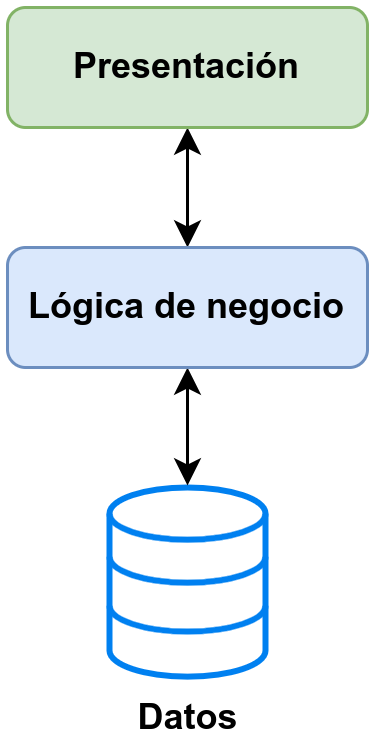
\includegraphics[width=0.25\linewidth]{capas.png}
\end{center}

\begin{itemize}
    \item \textbf{Capa de presentación}: Es la que ve el usuario (también se la denomina «capa de usuario»), presenta el sistema al usuario, le comunica la información y captura la información del usuario en un mínimo de proceso (realiza un filtrado previo para comprobar que no hay errores de formato).

    También es conocida como interfaz gráfica y debe tener la característica de ser «amigable» (entendible y fácil de usar) para el usuario. Esta capa se comunica únicamente con la capa de negocio.

    Hoy en día lo habitual es que hagamos uso de servicios web, por lo que la capa de presentación es \textbf{la web que estamos visualizando}. En el caso de aplicaciones móviles, es \textbf{la propia aplicación que tenemos instalada en el dispositivo}.

    \item \textbf{Capa de negocio}: es donde residen los programas que se ejecutan, se reciben las peticiones del usuario y se envían las respuestas tras el proceso. Se denomina capa de negocio (e incluso de lógica del negocio) porque es aquí donde se establecen todas las reglas que deben cumplirse.

    Esta capa se comunica con la capa de presentación, para recibir las solicitudes y presentar los resultados, y con la capa de datos, para solicitar al gestor de base de datos almacenar o recuperar datos de él. También se consideran aquí los programas de aplicación.

    En este tipo de arquitecturas, esta capa es la que se denomina \textbf{\textit{backend}}, y lo habitual es que sea un sistema al que llamamos a través de una \href{https://es.wikipedia.org/wiki/API}{API} (del inglés, \textit{application programming interface}, o interfaz de programación de aplicaciones).

    \item \textbf{Capa de datos}: es donde residen los datos y es la encargada de acceder a los mismos. Está formada por uno o más gestores de bases de datos que realizan todo el almacenamiento de datos, reciben solicitudes de almacenamiento o recuperación de información desde la capa de negocio.
\end{itemize}


\chapter{Escalado vertical vs horizontal}

Teniendo en cuenta todo lo dicho hasta ahora, cuando un sistema empieza a tener problemas de rendimiento deberemos abordar el problema y plantearnos cómo solucionarlo. De no hacerlo, se corre el peligro de que el servicio se vea interrumpido y por tanto perder tiempo de trabajo.

Antes de realizar ninguna modificación habría que analizar qué es lo que está sucediendo (para ello es importante tener un buen sistema de monitorización), y de esta manera saber en qué punto existe el problema y así poder solucionarlo.

Dependiendo de las decisiones tomadas durante la instalación, y tras lo visto previamente, podremos abordarlo de dos maneras diferentes.

\section{Escalado vertical}

Cuando se escala verticalmente un sistema lo que se va a realizar es el \textbf{añadir más recursos al nodo que está teniendo problemas}. Tras el análisis previo realizado se añadirán los recursos necesarios (más RAM, discos duros más rápidos, aumentar el número de procesadores/cores).

Comúnmente también se dice “meter más hierro”, porque antiguamente lo que se hacía era incrementar los recursos hardware del sistema. Hoy en día en sistemas virtualizados, estos recursos se pueden modificar, dependiendo del virtualizador, en caliente, por lo que no sería necesario reiniciar el servicio.

Es el sistema más simple, ya que incrementando los recursos se espera que el problema se apacigüe o desaparezca, aunque esto no tiene por qué ser siempre así.



    \part{Odoo}
    \chapter{Introducción}
\href{https://es.wikipedia.org/wiki/Odoo}{Odoo}, antes conocido como \textit{OpenERP} es un software de planificación de recursos empresariales con licencia dual. Existe una versión de código abierto y una versión con licencia comercial con características y servicios exclusivos.

Odoo también cuenta con un apartado de CRM (en inglés \textit{customer relationship management}, o gestión de relaciones con el cliente), pudiendo también crear una web de comercio electrónico, facturación, ...


\chapter{Instalación}

Tal como hemos visto en el tema anterior, la instalación de un sistema se puede realizar de distintas maneras, por lo que deberemos atender a las necesidades del proyecto para realizar una instalación adecuada.

En nuestro caso, se va a optar por realizar una instalación a través de servicios Docker, de esta manera podemos realizar pruebas con distintas versiones (tanto de Odoo como de la base de datos).

\infobox{La alternativa sería realizar la instalación en una máquina virtual o haciendo uso de los distintos instaladores que existen en la \href{https://www.odoo.com/es_ES/page/download}{web oficial}}

Para realizar la instalación seguiremos las indicaciones que aparecen en la web de \href{https://hub.docker.com/_/odoo}{Docker Hub} haciendo pequeñas modificaciones.

\section{Servicios independientes}

Es el sistema más básico, que requiere de levantar dos contenedores Docker:
\begin{itemize}
    \item Contenedor de base de datos \textbf{PostgreSQL}. Podremos elegir entre las distintas versiones del gestor de base de datos, pero haremos caso a las recomendaciones de la web. Habría que tener especial cuidado con el usuario y la contraseña que utilizamos.

    En este caso también se ha expuesto el puerto 5432 que es el puerto por defecto de PostgreSQL:

\begin{mycode}{Crear y arrancar el contenedor de la base de datos}{console}{}
ruben@vega:~$ docker run -d -e POSTGRES_USER=odoo \
-e POSTGRES_PASSWORD=odoo -e POSTGRES_DB=postgres \
-p 5432:5432 --name odoo_db postgres:15
\end{mycode}

    \item Contenedor con el propio \textbf{Odoo}. Este contenedor tendrá los servicios y librerías necesarias para poder hacer funcionar la aplicación web.

\begin{mycode}{Crear y arrancar el contenedor de la base de datos}{console}{}
ruben@vega:~$ docker run -p 8069:8069 --name odoo \
--link odoo_db:db -t odoo
\end{mycode}
\end{itemize}


\section{Docker Compose}

Docker Compose es una herramienta para correr servicios multi-contenedor y se crea a través de un fichero en formato YAML. Es una manera de crear,parar,reconstruir una arquitectura de servicios de manera rápida y sencilla.

Se debe crear un fichero \configfile{compose.yaml} y lo ideal es que esté dentro de un directorio con el nombre del “stack de servicios”, ya que coge el directorio como parte del nombre a la hora de crear los contenedores.

\begin{mycode}{Contenido de fichero compose.yaml}{yaml}{}
version: '3.1'
services:
  web:
    image: odoo:16.0
    depends_on:
      - db
    ports:
      - "8070:8069"
  db:
    image: postgres:15
    environment:
      - POSTGRES_DB=postgres
      - POSTGRES_PASSWORD=odoo
      - POSTGRES_USER=odoo
    ports:
      - "5433:5432"
\end{mycode}

Para arrancar los servicios se realiza, desde el mismo directorio donde se encuentra el fichero, con el siguiente comando

\begin{mycode}{Levantar docker compose}{console}{}
ruben@vega:~$ docker compose up
\end{mycode}

\errorbox{En Julio del 2023 se migró a Compose v2, tal como se indica en la \href{https://docs.docker.com/compose/}{web oficial}. Dependiendo de la versión que tengamos instalada será “docker compose up” o “docker-compose up”}


\section{Herramientas extra}
Para poder acceder a la base de datos podemos hacer uso de un cliente externo. De esta manera no tendremos que entrar al contenedor y tendremos un interfaz gráfico con el que poder administrarla.

Podemos utilizar:
\begin{itemize}
    \item \textbf{DBeaver}: Es una aplicación de escritorio que permite conectarnos a distintos SGBDs. Existe versión \href{https://dbeaver.io/}{community} y otra con \href{https://dbeaver.com/buy/}{licencia} que permite también conectarse a bases de datos NO-SQL.

    \item \textbf{\href{https://www.pgadmin.org/}{pgAdmin}}: Es una aplicación que permite administrar PostgreSQL a través del servidor web.
\begin{mycode}{Crear y arrancar el contenedor pgAdmin}{console}{}
ruben@vega:~$ docker run -p 8090:80 \
-e 'PGADMIN_DEFAULT_EMAIL=user@domain.com' \
-e 'PGADMIN_DEFAULT_PASSWORD=SuperSecret' \
--name pgadmin4 -d dpage/pgadmin4
\end{mycode}
\end{itemize}

% METER APLICACIONES DE SOPORTE????


    \part{Cómo crear una API}
    \chapter{Introducción a Laravel}

\href{https://laravel.com/}{Laravel} es un \textit{framework} para crear aplicaciones y servicios web haciendo uso del lenguaje de programación \href{https://es.wikipedia.org/wiki/PHP}{PHP}, buscando la simplicidad y evitar el “\textit{spaghetti code}”. Hace uso de la arquitectura “modelo-vista-controlador” (MVS) y es un proyecto de código abierto.

\section{Características}
Entre las características que tiene Laravel, se pueden destacar:

\begin{itemize}
    \item Sistema de enrutamiento, también RESTful.
    \item Motor de plantillas web llamado \href{https://laravel.com/docs/10.x/blade}{Blade}. Nos permite:
    \begin{itemize}
        \item Crear plantillas que pueden incluir otras plantillas.
        \item Hacer uso de PHP dentro de las plantillas.
        \item Permite cachear las plantillas hasta que se modifiquen.
    \end{itemize}
    \item Creador de queries a la base de datos llamada \href{https://laravel.com/docs/10.x/queries}{Fluent}.
    \item \href{https://laravel.com/docs/10.x/eloquent}{Eloquent} como ORM (\textit{object-relational mapper}).
    \item Uso de “\textit{migrations}” para crear la base de datos a modo de sistema de control de versiones.
    \item Sistema de enrutado de la aplicación para relacionar rutas de acceso con controladores.
    \item Posibilidad de usar “semillas” (en inglés “\textit{seeds}”) en la base de datos para importar datos, ya sea de test o datos iniciales necesarios.
    \item Permite hacer uso de paquetes de \href{https://getcomposer.org/}{Composer}.
    \item Soporte para usar servicios de caché.
    \item Posibilidad de paginación automática.
\end{itemize}

Estas características las iremos utilizando para crear nuestro primer proyecto y para posteriormente aprender a crear una API que podrá ser accedida desde cualquier tipo de aplicación: un interfaz web, una aplicación móvil, desde línea de comandos...
    \chapter{Crear primer proyecto en Laravel}

A la hora de crear un proyecto en Laravel lo primero que deberíamos hacer es visitar la \href{https://laravel.com/docs/10.x/installation}{documentación}, ya que nos dará distintas opciones dependiendo del sistema operativo en el que nos encontremos. Aparte, podremos ver si ha habido cambios desde la última vez que hayamos creado un proyecto.

\section{Servicios a utilizar}

Antes de crear el proyecto, debemos tomar una serie de decisiones para nuestro \textit{stack} de aplicación. Laravel cuenta con distintos servicios, algunos de ellos necesarios y otros optativos, por lo que deberemos tenerlos en cuenta.

Los servicios entre los que deberemos decidir son:

\begin{itemize}
    \item \textbf{Sistema Gestor de Base de Datos a utilizar}: Laravel permite el uso de distintos sistemas de bases de datos relacionales como son \href{https://dev.mysql.com/downloads/mysql/}{MySQL}, \href{https://www.postgresql.org/}{PostgreSQL} y \href{https://mariadb.org/}{MariaDB}. Por defecto hace uso de \textbf{MySQL}.
    \item \textbf{Sistema de caché}: Podemos hacer uso de distintos sistemas para cachear desde la sesión a información obtenida de la base de datos y también HTML. Por defecto, \textbf{Laravel cachea la sesión en el sistema de ficheros}, pero eso puede ser lento, por lo que se permite hacer uso de sistemas \textbf{clave-valor} para el almacenamiento de información para acelerar el rendimiento de la aplicación web. Se puede elegir \href{https://www.memcached.org/}{Memcached} o \href{https://redis.io/}{Redis} entre otros.
\end{itemize}

Otros servicios que podemos instalar y que nos darán ciertas funcionalidades son:

\begin{itemize}
    \item \textbf{\href{https://github.com/axllent/mailpit}{Mailpit}}: Es un sistema para controlar los emails que envía nuestra aplicación durante el desarrollo. En lugar de enviarlos a las cuentas finales, se quedan almacenados y se pueden visualizar a través de una web que a modo de buzón de correo. También ofrece una API.

    \item Uso de  \href{https://min.io/}{MinIO} para simular el \textbf{almacenamiento en la nube S3}. De esta manera no tendremos que crear un Bucket de pruebas.

    \item Sistema de \textbf{búsqueda \textit{full-text}} en la base de datos gracias a \href{https://laravel.com/docs/10.x/scout#introduction}{Scout} y haciendo uso del backend \href{https://www.meilisearch.com/}{MeiliSearch}.

    \item Creación y automatización de \textbf{tests} utilizando \href{https://www.selenium.dev/}{Selenium}.
\end{itemize}

Estas son algunas de los servicios que podríamos configurar antes de comenzar a crear nuestra aplicación. Para comenzar de manera sencilla nos centraremos únicamente en la elección de la base de datos, dejando el resto de servicios para más adelante.


\section{Instalación mediante Sail y Docker}

En la \href{https://laravel.com/docs/10.x/installation}{documentación} de Laravel nos explica cómo realizar la instalación de distintos modos teniendo en cuenta el sistema operativo, los servicios iniciales que nos interesan y el sistema de instalación que mejor se adapte a nuestro entorno.

%En este apartado se van a explicar dos modos:
%\begin{itemize}
%    \item Haciendo uso del método oficial y \textbf{Laravel Sail}, que nos permitirá elegir los servicios que necesitamos y que creará el proyecto haciendo uso de contenedores Docker.
%
%    \item Instalando Laravel utilizando \href{https://getcomposer.org/}{Composer}, que también es un método oficial, pero en este caso vamos a crear nosotros el contenedor Docker del servicio web y de base de datos. En caso de tener un entorno de PHP con Composer local, quizá no interesa realizar la creación del contenedor Docker.
%\end{itemize}
%
%Ambos métodos son igual de válidos y al final obtendremos un sistema similar.

%\subsection{}

El sistema es similar utilizando GNU/Linux, Windows y MacOS, con la salvedad de que en Windows deberíamos instalar Docker Desktop y \textit{Windows Subsystem for Linux} (WSL).

Para realizar la instalación sólo vamos a elegir tener el servicio de MySQL, para simplificarlo, tal como se ha comentado previamente. Para ello, deberemos ejecutar lo siguiente en el directorio donde nos interese crear el directorio del proyecto.

\begin{mycode}{Titulo}{console}{{\small }}
ruben@vega:~$ curl -s "https://laravel.build/example-app?with=mysql" | bash
\end{mycode}

Este comando lo que va a hacer es descargarse un script que va a ejecutar lo siguiente:
\begin{enumerate}
    \item Se va a asegurar que Docker está corriendo
    \item Va a levantar un contenedor con la imagen “laravelsail/php82-composer” que nos va a crear un directorio llamado \configdir{example-app} con un proyecto limpio de Laravel usando MySQL como SGBD.
    \item Si no tenemos la imagen de MySQL la descarga.
\end{enumerate}





\section{Configuración inicial}


    \chapter{Crear API}
    %Cómo crear una API con Laravel
%     - crear proyecto
%    - crear esquema E/R
%    - crear controlador
%    - crear funciones


    % ESTO IGUAL EN DESARROLLO DE INTERFACES?
%    \part{Crear frontend con Angular}
%    - crear proyecto
%    - crear primeras vistas
%    - llamar a la API

    \part{Introducción a Docker}
    \graphicspath{{../../../otros/Docker/}}
    \chapter{Introducción}

Hoy en día es muy habitual hacer uso de un sistema de contenedores, como es \href{https://docs.docker.com/}{Docker}, en el mundo del desarrollo de \textit{software}. Este sistema trae consigo una serie de ventajas que veremos más adelante, que nos permite asegurar, entre otras cosas, que las versiones utilizadas en el entorno de producción es la misma que durante las etapas de desarrollo.

En este documento se va a explicar cómo realizar la instalación y configuración de un sistema basado en contenedores Docker para poder arrancar servicios, y ciertas configuraciones que son necesarias conocer.

\chapter{Sistemas de contenedores}

\section{Un poco de historia}

\section{Contenedores vs. Máquinas virtuales}

El uso de máquinas virtuales está muy extendido gracias a que cada vez es más sencillo crearlas. Esto no quiere decir que siempre sea la mejor opción, por lo que  se va a realizar una comparativa teniendo en cuenta distintos aspectos a la hora de realizar un desarrollo con máquinas virtuales y con sistemas de contenedores.


\subsection{Infraestructura}

La creación de máquinas virtuales (a través de sistemas como VirtualBox) nos permite crear entornos aislados en los que poder instalar el Sistema Operativo que más nos interese y con ello poder instalar el software y los servicios que necesitemos.

Esto supone una gran ventaja, pero a la vez un gasto de recursos que podríamos utilizar para hacer uso en los servicios que queremos correr.

\begin{center}
    \includegraphics[width=0.9\linewidth]{img/docker/docker\_vs\_vm.png}
    \captionof{figure}{Infraestructura Máquinas Virtuales vs Docker}
\end{center}


En la imagen se puede apreciar una comparativa diferenciando cómo quedaría una infraestructura de 3 aplicaciones levantadas en distintas máquinas virtuales o en distintos contenedores.

Tal como se puede ver en la imagen, \textbf{al tener cada servicio en una máquina virtual separada}, se va a tener que virtualizar todo el Sistema Operativo en el que se encuentre, con el consiguiente \textbf{coste de recursos (memoria RAM y disco duro) y con el coste en tiempo de tener que realizar la configuración y securización del mismo}.

\infobox{\textbf{Usando contenedores la infraestructura se simplifica notáblemente}}

Por otro lado, en un sistema de contenedores, cada contenedor es un servicio aislado, en el que sólo tendremos que preocuparnos (en principio) de configurar sus parámetros.


\subsection{Ventajas durante el desarrollo}

A la hora de desarrollar una aplicación es habitual hacer pruebas utilizando distintas versiones de librerías, \textit{frameworks} o lenguajes de programación. De esta manera, podremos ver si nuestra aplicación es compatible.

Cuando se hace uso de una máquina virtual dependemos de las versiones que tiene nuestra distribución y es posible que no podamos instalar nuevas versiones u otras versiones en paralelo.

Por ejemplo, la última versión de PHP actualmente es la 8.2.4 y de Apache la 2.4.56:

\begin{itemize}
    \item En\textbf{ Debian 11} sólo se puede instalar PHP 7.4 y Apache 2.4.54.
    \item En \textbf{Ubuntu 22.04} la versión de PHP es la 8.1 y la de Apache la 2.4.52.
\end{itemize}

Con Docker, podremos levantar contenedores con distintas versiones del servicio que nos interese en paralelo para comprobar si nuestra aplicación/servicio es compatible.

\infobox{\textbf{Con Docker es posible levantar entornos/servicios con distintas versiones en paralelo}}

Por otro lado, si un desarrollador quiere utilizar un sistema operativo distinto, no se tendrá que preocupar de si su distribución tiene las mismas versiones. O en el caso de usar Windows/Mac, no tener que estar realizando instalaciones de las versiones concretas.


\subsection{Ventajas durante la puesta en producción}
Ligado al apartado anterior, durante la puesta en producción es obligatorio hacer uso de las mismas versiones utilizadas durante el desarrollo para asegurar la compatibilidad.

\errorbox{\textbf{Para asegurar la compatibilidad en producción, siempre se debe usar la misma versión de los servicios que en desarrollo}}

Si tenemos un servidor que no está actualizado, o en el mismo servidor tenemos distintas aplicaciones que requieren utilizar distintas versiones de software, en un entorno de máquinas virtuales se hace muy complejo, ya que lo habitual será tener que instalar nuevas máquinas virtuales.

\warnbox{\textbf{No siempre es posible tener distintas versiones del mismo software en un mismo servidor}}

En un entorno con contenedores, al igual que se ha comentado antes, esto no es problema.

\subsection{Rapidez en el despliegue}

Ligado a todo lo anterior, realizar el despliegue de un entorno de desarrollo/producción es más rápido utilizando contenedores, dando igual el sistema operativo en el que nos encontremos.

\infobox{El despliegue con contenedores es más rápido.}

Más adelante se verá cómo realizar el despliegue de distintos servicios haciendo uso de un único comando.


\chapter{Docker}




\chapter{Configuración básica}


\section{Primer arranque}


%    \graphicspath{{../../../anexos/sistemas_monitorizacion/img/}}
%    \hypertarget{sistemas_de_monitorizacion}{}

\chapter{Sistemas de Monitorización}

El sistema de monitorización se encarga de recopilar información acerca del estado de los servidores de una infraestructura. Entre las métricas y datos que debe recopilar se encuentran:

\begin{itemize}
    \item \textbf{Estado del servidor}: cantidad de RAM utilizada, estado de los discos duros, carga del servidor, sistema de ficheros,  …
    \item Estado de los \textbf{servicios que tiene el servidor}: servidor web, número de procesos que tiene, bases de datos, conexiones existentes, cola de correos electrónicos para enviar si es un servidor de correo, … Dependiendo del servicio habrá que realizar unas comprobaciones u otras.
    \item \textbf{Infraestructura en la que se encuentran}: estado de la red, conexión a otros servidores, …
    \item \textbf{Estado del clúster}: en caso de que el servidor pertenezca a un clúster, hay que comprobar que el clúster se encuentra en perfecto estado.
    \item \textbf{Dependencias externas}: un servidor puede depender a su vez de otros, o de servicios externos, que deben de estar funcionando de manera correcta.
\end{itemize}

Normalmente en la monitorización actúa un \textbf{agente} (o servicio) instalado en el equipo monitorizado que obtiene la información requerida que se envía a un servidor central que recopila la información de toda la infraestructura monitorizada.

Esta información suele ser almacenada durante un periodo de tiempo determinado (un año, por ejemplo) para poder ser usada y comparar la situación de los servidores a lo largo del tiempo. Gracias a esta comparación temporal \textbf{se puede llegar a predecir el estado del servidor} a unos días/semanas vista y evitar problemas antes de que sucedan (no tener espacio en discos duros, mal funcionamiento de servicios por falta de RAM, … ).

\infobox{\centering\textbf{La monitorización de servicios y equipos dentro de una infraestructura debe considerarse parte del proyecto, ya que es una parte muy importante de cara al mantenimiento del mismo.}}

\section{Monitorización de servidores}
Es habitual que los sistemas de monitorización funcionen en base a plantillas, que posteriormente se pueden asociar a los servidores monitorizados. Estas plantillas contendrán los servicios que deben ser monitorizados en cada tipo de servidor, ya que no es lo mismo monitorizar un servidor web o un servidor con un SGBD.

Para monitorizar un servidor lo habitual suele ser realizar las siguientes operaciones:

\begin{itemize}
    \item \textbf{Comprobar conectividad con el servidor}: suele ser habitual que los servidores estén fuera de nuestra red (en un proveedor de Internet, en un cliente, en otra oficina…), por lo que es necesario que exista conectividad de alguna manera para poder realizar la monitorización. En caso de no estar en nuestra red, el uso de una VPN es lo más utilizado.
    \item \textbf{Instalar un agente en el propio servidor}: Será el encargado de recopilar la información necesaria para mandarla al servidor central. Dependiendo del sistema de monitorización utilizado, necesitaremos un tipo de agente u otro. Algunos se encargan de realizar todas las comprobaciones y otros llaman a otros programas para realizar las comprobaciones y después mandar el resultado al servidor central.
    \item \textbf{Dar de alta el servidor en el sistema centralizado}: Tal como se ha dicho previamente, lo habitual es contar con un sistema centralizado en el que se tendrán todos los servidores y el estado de las comprobaciones realizadas. De ser así, habrá que darlo de alta, y para ello se necesitará:

    \begin{itemize}
        \item \textbf{Nombre del servidor}: Un nombre que a simple vista identifique el servidor. Suele ser habitual poner el nombre del cliente también, y/o el tipo de servicio que preste.
        \item \textbf{IP del servidor}: Para poder realizar la conexión al servidor.
        \item \textbf{Plantillas asociadas}: En caso de utilizar un sistema que utilice plantillas, al dar de alta el servidor se le aplicarán las plantillas necesarias para que realicen todos los checks oportunos. Por ejemplo: plantilla de Servidor Linux + plantilla de Servidor web + Plantilla de MySQL.
        \item \textbf{Puerto de conexión}:  Los agentes de monitorización suelen contar con un puerto que queda a la escucha. Si hemos cambiado el puerto, habrá que indicarlo a la hora de dar de alta.
        \item \textbf{Otras opciones}: Dependiendo del sistema de monitorización se podrán añadir muchas más opciones, como por ejemplo:
        \begin{itemize}
            \item \textbf{Servidores de los que se depende}: Imaginemos que el servidor monitorizado depende a su vez de un router que también está monitorizado. Si el router cae, no llegaríamos al servidor, por lo que realmente es una caída por dependencia, aunque el servidor puede estar funcionando de manera correcta. Esto nos puede permitir crear “árboles de dependencias” de servidores.
            \item \textbf{Periodos de monitorización}: Lo habitual es que un servidor esté monitorizado 24x7, pero quizá nos interese realizar cambios y que sólo se monitorice en unas horas determinadas (quizá el resto del tiempo está apagado).
            \item …
        \end{itemize}
    \end{itemize}
\end{itemize}

\section{Funcionamiento de la monitorización}
Para conocer cómo funciona un sistema de monitorización lo mejor es que tomemos como ejemplo un tipo de servicio que queremos monitorizar. Como ejemplo se puede tomar las comprobaciones que queremos realizar a un SGBD (Sistema Gestor de Bases de Datos).

No será lo mismo realizar la monitorización de un servidor MySQL o de un Oracle, pero las comprobaciones que queremos realizar en ellos deberían ser similares. Vamos a querer realizar la monitorización de las mismas comprobaciones: estado de las tablas en memoria, número de hilos en ejecución, número de \textit{slow\_queries}, …; pero los scripts ejecutados serán distintos.

\infobox{\textbf{La monitorización dependerá del propio servicio que vayamos a monitorizar.}}

A continuación se puede ver el estado de un servidor monitorizado a través del sistema de monitorización \href{https://www.centreon.com/}{Centreon}:

\begin{tcolorbox}[colback=white,title=Servidor monitorizado en Centreon]
  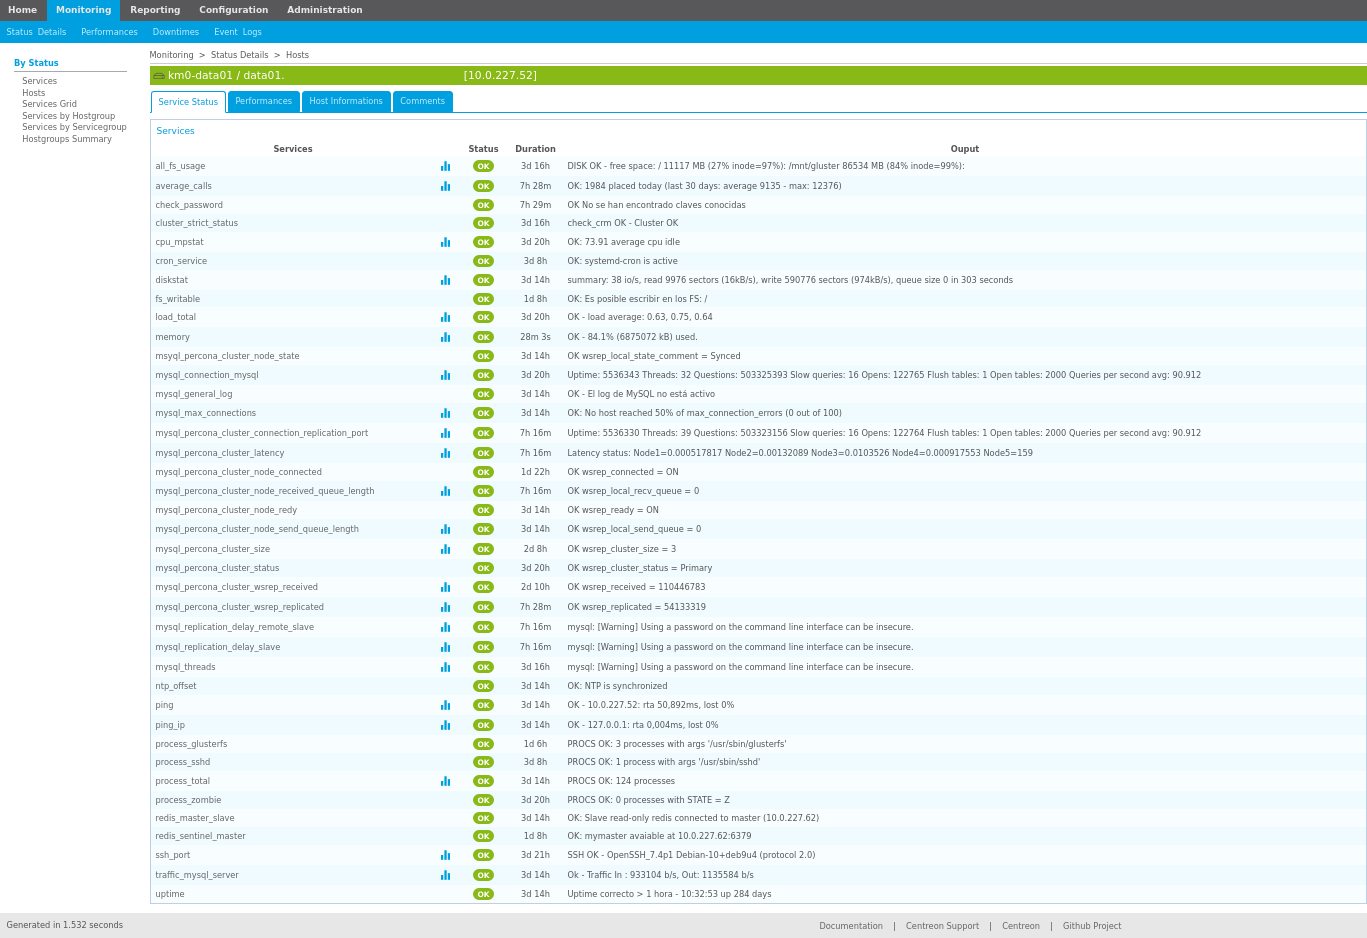
\includegraphics[width=\linewidth]{centreon.png}
\end{tcolorbox}



En la imagen anterior se puede comprobar un número de \textbf{\textit{checks}}, o comprobaciones, que se están realizando sobre un servidor concreto. Cada fila es una comprobación y contienen:

\begin{itemize}
    \item \textbf{Nombre del check/servicio}: Un nombre para identificar qué es lo que se está comprobando con el check.
    \item \textbf{Icono para mostrar gráficas}: Algunos checks recibirán información que puede ser graficada para así poder observar patrones en el comportamiento del servidor. Por ejemplo: cantidad de RAM ocupada, número de procesos en el sistema, número de conexiones a un servidor, …
    \item \textbf{Estado del check}: Normalmente, tras realizar la comprobación, el check termina con uno de los siguientes resultados:
    \begin{itemize}
        \item \textbf{OK}: El resultado obtenido es el correcto.
        \item \textbf{Warning}: El resultado obtenido está entre los márgenes de peligro. Es posible que de seguir así pase al estado siguiente:
        \item \textbf{Crítico}: El servicio devuelve un estado que es considerado crítico, lo que puede hacer que llegue a mal funcionamiento del mismo, o incluso que el servidor comience a dejar de funcionar (imaginemos que el servidor está con el 90\% de la RAM ocupada o de disco duro ocupado).
        \item \textbf{Indeterminado}: Por alguna razón, el \textit{check} no se ha realizado, o el valor devuelto es indeterminado o no se puede saber en qué otro estado situarlo.
    \end{itemize}
    \item \textbf{Duración del estado}: Para conocer cuánto tiempo lleva en el estado la comprobación obtenida. Lo ideal es que nunca haya estados que no sean OK y por lo tanto la duración de los mismos sea lo más alta posible.
    \item \textbf{Valor devuelto por la monitorización}: El valor real devuelto por la comprobación realizada. En base a este resultado se puede realizar las gráficas mencionadas previamente.
\end{itemize}

\infobox{\textbf{El estado del servicio dependerá del valor devuelto por la monitorización.}}

Este resultado se cotejará con los valores que hayamos puesto para que sea considerado OK, Warning o Critical. Es decir, \textbf{en algunos casos el estado del servidor depende de los valores devueltos y de la baremación que le hayamos otorgado}.

Pongamos como ejemplo la monitorización de un SGBD:
\begin{itemize}
    \item \textbf{El servicio del SGBD está funcionando}: Ahí no hay baremación posible. Si el servicio no está arrancado, es lógico pensar que el estado es crítico y que por tanto hay que ver qué ha ocurrido.
    \item \textbf{Número de conexiones en el SGBD}:  El resultado devuelto será un número entero (que podremos graficar para obtener patrones). En este caso, podemos decidir los rangos para que el resultado sea OK, Warning o Critical. Es decir, si el resultado obtenido está por debajo del umbral de Warning, el sistema considerará que el estado es OK. Si está en dicho rango, será Warning y si está en el rango de Critical, así lo indicará.
\end{itemize}

Esta baremación y \textbf{estos rangos} se suelen aplicar también en las plantillas de los servicios. Hay que entender que también \textbf{pueden ser modificados y personalizados para un servidor concreto}. No es lo mismo que un SGBD tenga 500 conexiones simultáneas si tiene 8Gb de RAM o si tiene 128Gb (en el primer servidor se puede considerar que es un estado crítico mientras que en el segundo es lo esperado).

Cuando un \textit{check} termina siendo un Warning o un Critical \textbf{es habitual que haya un sistema de alarmas configurado}. Dependiendo del sistema utilizado, notificará a los administradores mediante e-mail, mensajería instantánea, SMS, … para que realicen un análisis lo antes posible y solucionen el estado del servicio.

\infobox{\textbf{Los sistemas de monitorización suelen contar con un sistema de alarmas para que nos avise de los servicios caídos.}}


\subsection{Monitorización básica}
Tal como se ha comentado, en los servidores se suele realizar una monitorización del estado del mismo que suele ser común para todos, por lo que lo habitual suele ser tener una plantilla genérica para todos los servidores con la que se monitorizará:
\begin{itemize}
    \item Cantidad de RAM utilizada
    \item Cantidad de memoria virtual utilizada
    \item Carga de la CPU
    \item Espacio libre en las unidades de disco duro
    \item Estado del sistema RAID del servidor (en caso de tenerlo)
    \item Cantidad de usuarios conectados a la máquina
    \item Estado de puertos de conexión (SSH, por ejemplo)
    \item Latencia hasta llegar al servidor
    \item …
\end{itemize}

Es cierto que no será lo mismo monitorizar un sistema GNU/Linux o un sistema Windows (ya que puede variar alguno de las comprobaciones a realizar), pero el estado general que queremos conocer es el mismo. Por lo tanto, lo habitual es tener dos plantillas, una específica para servidores Windows y otra para GNU/Linux.


\subsection{Monitorización de Servicios}
Aparte de la monitorización básica comentada previamente, necesitaremos monitorizar el estado de los servicios que pueda tener el servidor propiamente dicho. Para ello, de nuevo, se crearía una plantilla específica para cada tipo de Servicio que podamos tener en nuestro servidor.

No será lo mismo monitorizar un servidor que tenga un servidor web, un servidor de base de datos, un proxy… O puede que el servidor cuente con todos esos servicios.

Es por eso que a la hora de realizar la monitorización de un servidor \textbf{es muy importante conocer qué funciones desempeña cada servidor en la infraestructura a la que pertenece} y analizar los servicios que tiene arrancados para posteriormente ser monitorizados.

\infobox{\textbf{Es muy importante conocer qué funciones desempeña cada servidor en la infraestructura a la que pertenece.}}


\section{Tipos de monitorización}
Existen varias maneras de realizar la monitorización de un servidor, y dependerá del gestor de monitorización que usemos (en caso de usar uno).

Es habitual que cuando nos referimos a sistemas de monitorización lo dividamos en dos grandes familias:
\begin{itemize}
    \item Monitorización Activa
    \item Monitorización Pasiva
\end{itemize}

Estas dos maneras de monitorización suelen ser excluyentes, aunque algunos sistemas de monitorización permiten ambas, por lo que nos puede interesar usar una u otra dependiendo de la situación.


\subsection{Monitorización pasiva}
En la monitorización pasiva el servidor (u objeto monitorizado) es el encargado de mandar la información de manera periódica al servidor central. El agente instalado se ejecutará como una tarea programada cada cierto tiempo (habitualmente unos pocos minutos) e informará de la situación cambiante, de haberla, al servidor central.

Esta manera de monitorización es utilizada también cuando no hay un servidor central. En este caso, si la comprobación ha sido incorrecta, podría mandar un mail al administrador del servidor.

\subsection{Monitorización activa}
Suele ser la manera habitual de proceder de los sistemas que cuentan con un servidor centralizado de monitorización. El servidor de monitorización se encarga de preguntar al servidor, a través de la conexión con el agente, por la comprobación de alguno de los checks, y el agente devuelve la información.

A continuación se puede observar las etapas que existen en un sistema de monitorización activa utilizando un servidor de monitorización central:

\begin{tcolorbox}[colback=white,title=Proceso de monitorización activa]
    \centering
    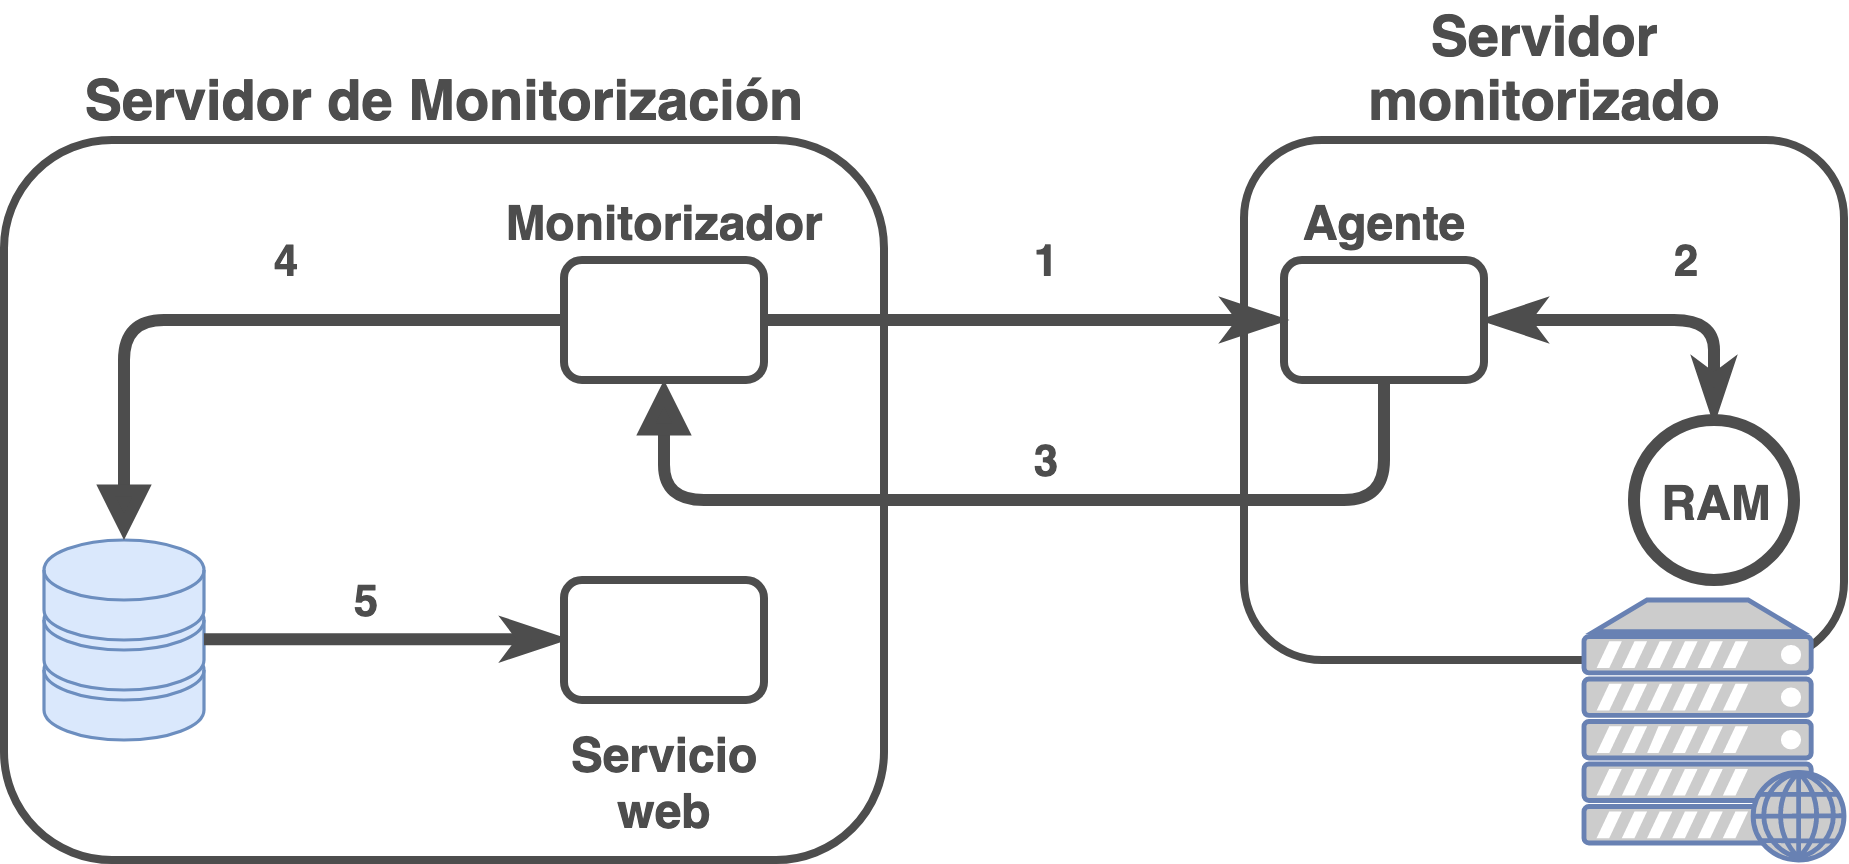
\includegraphics[width=0.6\linewidth]{monitorizacion_activa.png}
\end{tcolorbox}

Las etapas serían:
\begin{enumerate}
    \setcounter{enumi}{-1}
    \item El sistema de monitorización tiene un scheduler (o planificador) que decide cuándo tiene que realizar cada comprobación (normalmente, cada pocos minutos).
    \item El servicio encargado de monitorizar \textbf{establece conexión con el agente remoto} y le pide que compruebe un estado. En este ejemplo se ha optado por la RAM.
    \item El agente en el servidor que se quiere monitorizar recibe la notificación y realiza una \textbf{comprobación local} (normalmente llamando a scripts locales) para obtener la cantidad de RAM ocupada, total y libre que tiene
    \item El agente envía al sistema de monitorización el resultado obtenido en la ejecución de los scripts del paso anterior.
    \begin{enumerate}
        \item El monitorizador al recibir el resultado, lo coteja con los rangos de baremación que tiene y decide si el check está en estado OK, Warning o Critical.
        \item Lo habitual es que si el resultado del servicio no es OK, se ejecute en el servidor de monitorización algún tipo de alarma (ya sea enviar un mail, sistema de mensajería, … ) para notificar a los administradores.
    \end{enumerate}
    \item El sistema de monitorización guarda en una base de datos los resultados obtenidos para así poder realizar posteriores análisis o comprobaciones temporales de los mismos.
    \item Esos datos se suelen visualizar en una interfaz web, tal como hemos visto previamente.
\end{enumerate}

Estos pasos son ejecutados de manera continuada en el servidor de monitorización para cada comprobación que se realiza en cada uno de todos los servidores que se monitorizan. Por lo tanto, se entiende que el propio servidor de monitorización también tiene que ser monitorizado ya que es de vital importancia que su estado sea óptimo.

\subsection{Monitorización centralizada}
Como ya se ha comentado, es el sistema habitual de monitorización. Las ventajas que podemos obtener al hacer uso de este sistema son muchas, pero se pueden destacar las siguientes:
\begin{itemize}
    \item \textbf{Monitorización centralizada}: Aunque parezca obvio, el tener un único sistema en el que concentrar toda la información es muy útil y eficaz.
    \begin{itemize}
        \item La alternativa sería tener una monitorización distinta en cada servidor.
    \end{itemize}
    \item \textbf{Interfaz web}: Hoy en día suele ser habitual que los sistemas de monitorización tengan un servicio web en el que visualizar todos los datos obtenidos.
    \item \textbf{Sistema de plantillas}: De nuevo, es lo habitual, lo que hace que la gestión de monitorización de servidores sea más cómoda.
    \item \textbf{Gestión de usuarios}: Podremos tener usuarios que puedan ver unos servidores u otros, por lo que podemos tener equipos especializados en distintos grupos de monitorización y que sólo se enfoquen en ellos.
    \begin{itemize}
        \item Esto también es útil para dar acceso a los clientes a la monitorización de sus propios servidores.
    \end{itemize}
\end{itemize}

\subsection{Monitorización reactiva}
La monitorización reactiva se puede definir como el sistema de monitorización que no sólo se encarga de comprobar y recibir el estado de los servidores, si no que también reacciona a los mismos para tratar de solucionar los problemas encontrados. Tras esta definición está la idea de que \textbf{existen ciertos fallos recurrentes que no siempre necesitan la intervención humana para solucionarse}, y que por tanto, se puede tratar de ejecutar antes de que sea considerado un problema real.

Como \textbf{ejemplo sencillo} se puede poner \textbf{el espacio libre en disco duro}. Imaginemos que se comprueba que apenas hay espacio en el disco duro de un servidor. En este caso, el sistema de monitorización recibirá que el servidor \textbf{está al 99.95\%} de espacio ocupado, y por tanto, en lugar de notificar a un humano indicando el estado crítico, \textbf{el sistema reacciona de manera automática tratando de liberar espacio}. Se habrá configurado previamente que en la reacción de este error trate de borrar ficheros temporales, vaciar papelera, limpiar ficheros de caché de ciertas rutas … Una vez hecho esto, se volverá a comprobar el estado del servidor. Si el espacio ocupado en disco duro ha bajado y está en modo OK no habrá que hacer nada más, y se habrá evitado que un administrador tenga que realizar dicha tarea. Si por el contrario el estado sigue siendo incorrecto, el sistema notificará el error para que se realice un análisis y se solucione el problema.

Como \textbf{ejemplo extremo} (que no suele ser habitual configurarlo así), imaginemos que \textbf{la RAM consumida por un SGBD es muy alta} y esté poniendo en peligro el estado del servidor, se podría configurar para que \textbf{el sistema reaccione reiniciando el SGBD para que libere la RAM} y vuelva a prestar servicio.


\section{Gestores de monitorización}
Hoy día existen muchos sistemas de monitorización, y dependiendo de nuestras necesidades deberemos optar por uno u otro. A continuación se expondrán varios ejemplos de gestores de monitorización basados en Software Libre, aunque la gran mayoría de ellos cuentan con un sistema dual. Es decir, se puede descargar y montarlo en tu propio servidor o puedes contratar a la empresa para que ellos tengan el servicio central:
\begin{itemize}
    \item \textbf{\href{https://es.wikipedia.org/wiki/Nagios}{Nagios}}: Se puede considerar uno de los sistemas de monitorización más conocidos y del que se han basado otros. Generó mucha comunidad de administradores creando muchos scripts/plugins para hacerlos funcionar con él. Estos mismos scripts suelen ser utilizables en otros sistemas de monitorización.

    \item \textbf{\href{https://www.centreon.com/}{Centreon}}: Originalmente se creó como interfaz web para Nagios, pero poco a poco fue sustituyendo partes de Nagios hasta terminar siendo un sistema de monitorización completo. Existe la posibilidad de realizar la instalación por paquetes, descargar el sistema operativo en una ISO que te instala todo o incluso una máquina virtual con todo ya instalado y con configuración básica. (\href{https://demo.centreon.com/centreon/index.php}{Demo}).

    \item \textbf{\href{https://pandorafms.com/es/}{PandoraFMS}}: Sistema de monitorización creado por el español Sancho Lerena Urrea. Al igual que los anteriores, tiene sistema dual y la instalación se puede realizar por varios métodos.

    \item \textbf{\href{https://www.cacti.net/}{Cacti}}: Sistema más sencillo que los anteriores y habitualmente utilizado sólo en servidores sueltos, es decir, no de manera centralizada.

    \item \textbf{\href{https://munin-monitoring.org/}{Munin}}: Igual que el anterior, ideal para monitorizar unos pocos servidores, ya que no se puede considerar un sistema centralizado como los primeros. Ver \hyperlink{instalar_munin}{anexo de instalación de Munin}.
\end{itemize}

Existen otros sistemas de monitorización basados “en la nube”, cuya funcionalidad es similar a lo expuesto previamente. Para hacer uso de estos sistemas nos descargamos un agente, lo instalamos y se encargará de mandar la información a los servidores de la plataforma contratada. Lógicamente, dependiendo del gasto realizado obtendremos más o menos servicios. Entre este tipo de servicios se pueden destacar:
\begin{itemize}
    \item New Relic
    \item DataDog
\end{itemize}

\def\test{sgbd}
\ifx\test\@minititle
%% THIS PART ONLY IN SGBD BOOK
\else
%% THIS PART IN OTHER BOOKS
\fi

\clearpage
%
%    \part{Anexos}
%    \graphicspath{{../../../anexos/}}
%    \chapter{Glosario}

A continuación se expone un glosario de términos con sus correspondientes definiciones:

\begin{description}
    \hypertarget{altadisponibilidad}{}
    \item[Alta Disponibilidad:] Es un diseño de arquitectura de sistemas y la implementación que asegura que el servicio instalado y otorgado sea funcional sin que haya parada en el mismo. Esta arquitectura trata de que no haya ningún \hyperlink{spf}{\textit{single point of failure} (punto único de fallo)} en la misma.

    \hypertarget{cluster}{}
    \item[Clúster:] Se denomina clúster a un conjunto de ordenadores unidos entre sí mediante conectividad de red que actúan como si de un único servidor se tratara. Dependiendo del tipo de clúster que se va a crear, debe de ser pensado desde el diseño del servicio, ya que es la aplicación o servicio quién se encarga de crear el clúster (como ocurre con MySQL Cluster).

    \hypertarget{dependencia_software}{}
    \item [Dependencia de software:] Cuando se crea cualquier tipo de software lo habitual es hacer uso de otro software (librerías de seguridad, acceso a disco, codecs de vídeo, librerías 3D…) que son necesarias para el correcto funcionamiento de nuestro programa. Este otro software (que puede ser propio o ajeno) se denomina \textbf{dependencia}, ya que sin él, nuestro programa no funcionará y es necesario que exista en el sistema para hacer funciona nuestro programa.

    En las \hyperlink{distribucion_gnu_linux}{distribuciones GNU/Linux} se hace uso de los denominados \hyperlink{paquete_de_software}{paquetes de software} en los cuales se indican las dependencias que necesitan para funcionar y que por tanto se instalarán a la par que el programa elegido, por lo que nos aseguramos que el software instalado funcionará en cuanto termine la instalación.

    En caso de descargar un software ajeno de los \hyperlink{repositorio_de_software}{repositorios} oficiales de la distribución, es posible que necesitemos completar esas dependencias por nuestra cuenta, pero hoy en día es habitual que los creadores de software lo tengan en cuenta y esas dependencias estén en los repositorios oficiales.

    \hypertarget{distribucion_gnu_linux}{}
    \item [Distribución GNU/Linux:] Es una distribución de software basada en el núcleo Linux que incluye software \hyperlink{gnu}{GNU} para componer un Sistema Operativo que pueda ser utilizado por los usuarios. Cada distribución suele \hyperlink{paquete_de_software}{empaquetar el software} en un formato propio que aparte del propio software indica las \hyperlink{dependencia_de_software}{dependencias} de software que necesita para funcionar, por lo que hace que la instalación del software se realice de manera sencilla. El software de la distribución está almacenado en los \hyperlink{repositorio_de_software}{repositorios de software} oficiales de la distribución.

    Las distribuciones suelen estar orientadas para un uso generalizado, pero es cierto que algunas, por su historia o por su manera de entender el empaquetado de software, se necesitan más conocimientos, pero hoy en día no es lo habitual.

    Existen muchas distribuciones GNU/Linux, pero las que podríamos destacar son \hyperlink{ubuntu}{Ubuntu}, Debian, Red Hat y CentOS, que son las de mayor uso hoy en día a nivel profesional.

    \hypertarget{escalado_horizontal}{}
    \item[Escalado Horizontal:] Se llama escalado horizontal a la infraestructura que crece de manera horizontal añadiendo más servidores del mismo servicio. Estos servidores serán accesibles mediante un proxy o de manera directa, y todos contarán con el mismo servicio (web, base de datos, …). No confundir con un clúster, ya que la relación de los servidores en el escalado horizontal no tienen por qué ir en clúster.

    \hypertarget{escalado_vertical}{}
    \item[Escalado Vertical:] Es el incremento de hardware de un servidor. Supongamos que un servidor empieza a tener problemas de carga, pues con el escalado vertical se le añadiría más RAM, más procesador y/o discos duros más rápidos (en caso de ser una máquina virtual sería sencillo, en caso contrario habría que realizar la migración a un servidor nuevo).

    \hypertarget{gnu}{}
    \item[GNU:] Del acrónimo \textbf{GNU’s Not Unix} (GNU no es Unix) es un sistema operativo y un conjunto de programas libres cuyo origen surgió de la idea de crear un sistema operativo Unix basado en \hyperlink{software_libre}{Software Libre}.

    El desarrollo de GNU nació en 1983 por Richard Stallman comenzando por el compilador GCC, al que se fueron uniendo todo tipo de software y creando la Free Software Foundation (o FSF, fundación por el software libre) la cual creó la \hyperlink{licencias_libres}{licencia libre} más conocida actualmente: la \textbf{GPL} (GNU General Public License).

    El proyecto GNU avanzó en el tiempo y creó el kernel Hurd, pero bien es cierto que nunca llegó a ser funcional del todo y actualmente el kernel más utilizado es Linux, pero no es el único, ya que el software GNU también es usado en conjunto con otros kernels como son los \textbf{*BSD}, de ahí la importancia que cuando hacemos referencia al sistema operativo se haga uso de \hyperlink{gnu_linux}{GNU/Linux}.

    \hypertarget{gnu_linux}{}

    \itemimage{GNU/Linux:}{r}{0.21}
    {img/Gnulinux.svg.png}
    {\href{https://es.wikipedia.org/wiki/GNU/Linux\#/media/Archivo:Gnulinux.svg}{GNU/Linux: Wikipedia}}
    {
        Aunque comúnmente solemos llamar a las \hyperlink{distribucion_gnu_linux}{distribuciones} como “Linux” esto no suele ser correcto ya que en la distribución aparte del kernel va un conjunto enorme de software del proyecto GNU. Por lo tanto, lo ideal siempre es hacer uso del nombre completo GNU/Linux.

        El proyecto \hyperlink{gnu}{GNU} y sus herramientas y software son usados con otros kernels como son los *BSD en distribuciones como FreeBSD u OpenBSD. También existen versiones con kernel BSD para la distribución Debian, por lo que en ese caso sería “Debian GNU/BSD”.
    }


    \hypertarget{json}{}
    \item[JSON:] Es un formato de texto sencillo para el intercambio de datos. Aunque originalmente fue creado como notación de objetos para Javascript, su amplia utilización ha hecho que sea utilizado como alternativa a XML.


    \hypertarget{licencias_libres}{}
    \item[Licencias libres:] Una licencia de software es un contrato entre el creador (o el titular de los derechos de autor) del software y el usuario. Todo software que usamos suele exigir la lectura de esta licencia y es por ello muy importante conocer qué se puede y no se puede hacer con dicho software.

    Las licencias libres son aquellas que nos permiten hacer con el software lo que las cuatro libertades del \hyperlink{software_libre}{Software Libre} exige.

    Entre las licencias libres más utilizadas hoy en día están la GPL (General Public License del proyecto \hyperlink{gnu}{GNU}), la Apache License, algunas de las versiones de las licencias Creative Commons, …


    \hypertarget{linux}{}
    \item[Linux:] Creado originalmente por Linus Torvalds en 1991 y actualmente desarrollado por cientos de desarrolladores de todo el mundo, Linux es el núcleo (o kernel) gratuito y libre similar al núcleo de los sistemas operativos Unix.

    Comenzó como un proyecto personal de Linus (siendo estudiante universitario) para su ordenador 386 y actualmente está portado a \href{https://es.wikipedia.org/wiki/Portabilidad\_del\_n\%C3\%BAcleo\_Linux\_y\_arquitecturas\_soportadas}{decenas de plataformas hardware}. Es el proyecto más grande y ambicioso del \hyperlink{software_libre}{Software Libre}, aunque originalmente no se permitía el uso comercial del mismo (hasta la versión 0.12).

    Al poco tiempo de comenzar su desarrollo el proyecto \hyperlink{gnu}{GNU} lo adoptó como su kernel naciendo lo que actualmente conocemos como \hyperlink{gnu_linux}{GNU/Linux} y con ello cientos de \hyperlink{distribucion_gnu_linux}{distribuciones}.

    Es un núcleo de tipo monolítico que permite la carga de módulos en tiempo de ejecución


    \hypertarget{lts}{}
    \item[LTS:] Del inglés \textit{\textbf{L}ong \textbf{T}erm \textbf{S}upport} (en castellano “soporte a largo plazo”), es una característica en informática que hace referencia a versiones especiales de software que contarán con un soporte más largo del habitual, por lo que serán las versiones idóneas para usar en servidores.

    Estas versiones suelen contar con actualizaciones de seguridad, pero no con cambios notorios en la forma del software para fomentar la fiabilidad del mismo. Lo habitual es utilizar este tipo de versiones en servidores, que aunque puedan no tener las últimas modificaciones de las versiones más recientes del software, nos aseguramos la fiabilidad. Esto hace que tengamos que decidir si es necesario contar con las características de las últimas versiones (ya sea nuevos servicios, opciones nuevas, velocidad, … ) o si preferimos contar con una versión que tendrá un ciclo de vida más longevo pero con actualizaciones de seguridad.

    Es habitual verlo en proyectos de \hyperlink{software_libre}{Software Libre}, como ejemplos podemos tomar el kernel \hyperlink{linux}{Linux} (actualmente la versión 5.4.58 es la denominada LTS) y la distribución \hyperlink{ubuntu}{Ubuntu} (en este caso la versión 20.04).


    \hypertarget{paquete_de_software}{}
    \item[Paquetes de Software:] Un paquete de software no es más que una manera de poder distribuir el software creado. En \hyperlink{distribucion_gnu_linux}{distribuciones GNU/Linux} estos paquetes determinan las \hyperlink{dependencia_software}{dependencias} que necesitan para que su instalación sea lo más sencilla posible.

    Lo habitual es que estos paquetes estén gestionados mediante un sistema de gestión propio para conocer cuáles están instalados, sus dependencias, desinstalarlos de manera sencila...

    No sólo se usa en distribuciones GNU/Linux, ya que varios lenguajes de programación hacen lo propio para distribuir software en forma de paquetes. Como ejemplos:
    \begin{itemize}
        \item En distribuciones GNU/Linux tenemos APT, Yum, Zypper, Portage, ...
        \item En lenguajes de programación tenemos Gem para Ruby, Eggs para Python, CPAN en Perl, ...
    \end{itemize}


    \hypertarget{repositorio_de_software}{}
    \item[Repositorio de Software:] Se podría denominar repositorio como el almacén donde se guardan los \hyperlink{paquete_de_software}{paquetes de software}. Las \hyperlink{distribucion_gnu_linux}{distribuciones GNU/Linux} cuentan con sus repositorios oficiales, donde se almacena el software para cada versión que tiene la distribución.

    Aparte del software que podemos instalar, también cuentan con un índice para saber los paquetes y las versiones que se almacena en ellos. Este índice es necesario que lo actualicemos de manera periódica (en Ubuntu ejecutando: “apt update”) ya que gracias a él sabremos si tenemos que realizar actualizaciones de los paquetes instalados.

    También podemos utilizar repositorios externos al de la distribución, repositorios oficiales de un software por ejemplo, que nos permiten instalar la última versión de ese software sobre nuestra distribución. Cuando un paquete con el mismo nombre existe en distintos repositorios, siempre se instalará del repositorio que tenga la versión más nueva.

    No es buena práctica, y \textbf{está completamente desaconsejado}, mezclar repositorios de distribuciones distintas aunque el gestor de paquetes sea el mismo (usar repositorios de Debian en Ubuntu o viceversa).


    \hypertarget{spf}{}
    \item[Single Point of Failure:] O punto único de fallo, es un componente de un sistema que tras un fallo en su funcionamiento ocasiona un fallo global en el sistema completo, dejándolo inoperante. Un SPOF puede ser un componente de hardware, software o eléctrico.


    \hypertarget{software_libre}{}
    \item[Software Libre:] El movimiento del Software Libre fue creado por Richard Stallman a la par que creaba el proyecto \hyperlink{gnu}{GNU}. Para que un software sea considerado como Software Libre debe contener una \hyperlink{licencias_libres}{licencia libre} que debe otorgar las cuatro libertades siguientes:
    \begin{itemize}
        \item Libertad de usar el software para cualquier propósito.
        \item Libertad de estudiar el software y su funcionamiento interno (es por ello necesario poder acceder al código fuente).
        \item Libertad de distribuir el software con quien queramos.
        \item Libertad de poder modificar y mejorar el software según nos interese.
    \end{itemize}

    Es muy importante tener en cuenta que Software Libre no significa gratis, ya que en inglés el término viene de Free Software donde “Free” puede significar libre y gratis. Es cierto que la gran mayoría del Software Libre puede ser gratis, pero no todo el software gratis es Software Libre.


    \hypertarget{ssh_server}{}
    \item [SSH Server]: De \textbf{S}ecure \textbf{SH}ell, es el nombre de un protocolo y del programa (tanto servidor, como cliente) cuya función principal es la de acceder de manera remota a través de un canal seguro a un servidor.

    SSH permite no sólo la conexión a un servidor sino también la transferencia de ficheros y creación de túneles cifrados por los que pueden viajar otros protocolos. El puerto habitual de uso para este protocolo es el \textbf{22}.


    \hypertarget{systemd}{}
    \item [Systemd]: es un conjunto de demonios de administración de sistema, bibliotecas y herramientas diseñados como una plataforma de administración y configuración central para interactuar con el núcleo del Sistema operativo \hyperlink{gnu_linux}{GNU/Linux}.


    \hypertarget{ubuntu}{}

    \itemimage{Ubuntu:}{r}{0.21}
    {img/ubuntu.svg.png}
    {\href{https://es.wikipedia.org/wiki/Ubuntu}{Ubuntu: Wikipedia}}
    {
        Es una \hyperlink{distribucion_gnu_linux}{distribución de GNU/Linux} originalmente basada en Debian y creada por la compañía Canonical en el 2004. En su momento fue una de las distribuciones que apostaron por un sistema de instalación sencillo y con la intención de detectar el máximo hardware posible para acercarse a la gran cantidad de usuarios posibles.

        Hoy en día es una de las distribuciones más utilizadas tanto a nivel de escritorio como a nivel de servidores ya que cuenta con dos versiones separadas a la hora de realizar la instalación (aunque realmente es la misma distribución).

        Una de sus ventajas es la creación de versiones \hyperlink{lts}{LTS} cada dos años, que son versiones que garantizan su soporte técnico durante más tiempo por lo que supone una ventaja a la hora de realizar la instalación en servidores. Con ellos nos aseguramos que el software va a ser actualizado ante fallos de seguridad durante más tiempo que las versiones que no son LTS.
    }


\end{description}

\clearpage


\end{document}